\documentclass[12pt]{article}
\usepackage[margin=1in]{geometry}
\usepackage{amsmath}
\usepackage{amssymb}
\usepackage{graphicx}
\usepackage{caption}
\usepackage[colorlinks=true,urlcolor=red]{hyperref}
\usepackage{color}
\usepackage{enumerate}

\begin{document}
\title{Firewall Report}
\author{Akshay Dongaonkar (akd54)}
\maketitle

\section{Objective}

I am implementing a Linux based Firewall that mediates access between
two interfaces: a pipe to the Internet and a pipe to a protected, internal
network. Due to some exigent circumstances of which I've talked to the 
professor about, most of this design document is not implemented. Instead,
I will be talking about my design choices I am thinking of making now;
some of which will hopefully be implemented by tomorrow.

\section{Project Structure and Pipeline}

There are multiple components of this project that I tried to modularize 
into common library modules for reuse. For example, there is a module 
called parser that deals with file input and output. It has a function call
to read a rules file that codifies firewall rules, it has a function call 
to parse the /proc/net/tcp file to determine if a port is being used or not, 
and it at one point had code that iterated through a structure that stored 
log strings and wrote it to a file. \par

Then, my design decisions diverged. Initially, I wanted to have a 
multi threaded application that parallelized on the rule. I'd been working 
on that structure before I had to roll back my code as stated above. I had
ingress from an interface working with pcap loops with their own filter and
I wanted to extend that to multiple rules. I then wanted to compare this 
approach versus a stateful firewall which accepted every packet and 
looked up its validity within a hashtable. If not found, it would compare
against the rule set. My multi threaded approach would be very limited in
scale with respect to the number of rules, but it may have been easier to 
maintain and debug.

\section{Code and Data Structures}

Right now, there is a simple loop and a simple handler that grab packets off
of the currently used interface. 
The handler for the packets captured linearly checks against a filter string.
This is not extensible as there is only one rule in effect at all times. \par

The reason this happened was that I was basing a lot of my code from the
libpcap tutorial provided by
\href{http://yuba.stanford.edu/~casado/pcap/section3.html}{Stanford}.
I will be switching to a different architecture if I have enough time. \par

The current architecture I have in mind is to have multithreaded pcap capture
loops that grab packets that conform to their firewall rule.
The $n+1^{th}$ rule will specifically avoid packets captured by the $n$ rule
by careful use of the pcap filter expression. 
So, to make things easier for us, our firewall tries to match to the first 
rule, going top to bottom. \par

For a block rule, the captured packet references a special pcap handler that
simply does nothing to the packet.
For a pass rule, we reference a handler that injects the packet to our internal
network interface port.
This will give us most of the functionality that we need for our firewall.
For our DMZ, we have its rules at the top of our rule set.
We then have our capture loop reference a handler that forwards the packet
to the DMZ interface port. \par

However, this will not really scale.
We need a way to maintain states of connections so we do not have handle packet
analysis at every packet.
For large (elephant) streams, this would be very cumbersome.
I am not completely sure as to how I'm going to implement state with my 
pre-existing code structure. \par

In addition to handling the flows within the firewall, we still need other
structures to implement functionality as required by the project.
We need an ARP resolution protocol,
we need a NAT function for maintaining duplex connections,
and a flexible interface handler. \par

The NAT function is partially implemented as we parse our system files to 
determine open TCP ports. We also have functions that guarantee that the port
value it returns is not in use at the time of the return. This is done by 
keeping a bit vector of open ports from the system tcp files. Given this,
we can route flows with some NAT mode and store mappings in a hashtable. \par
The hashtable being used is the same one written for HW2. Considerable work
has been done to ensure non-segfaulting behavior within the hashtable so it
can be reused in multiple places in this project. \par
As for the ARP module, where we bind ARP requests for IP's to our address,
this is something that can be implemented and unit tested apart from the firewall.
This is the next item that will be implemented. \par
As for the multiple interface handler, this is something that will probably 
not be implemented. Right now, every interface is hard-coded and switching between
them may break dependencies that I do not know of. If it is possible to run,
then there will be a configuration file that will multiplex between the different
interfaces that will be captured during initialization. 

\section{Testing Strategy}

The testing strategy with my previous code setup was as follows. 
I was going to be using my HP laptop which runs Ubuntu 14.04 LTS.
I was going to capture packets from my \texttt{wlan0} interface to feed to my firewall.
Once the packets are ingested by the program,
the firewall will analyze the packets and match against rules
as described in the aforementioned section.
My firewall would then route the packet to an output interface. \par

To verify the rules worked, I would check against packets using Wireshark.
A picture of a sample Wireshark capture all is shown in Figure 1. \\
\begin{figure}[h]
	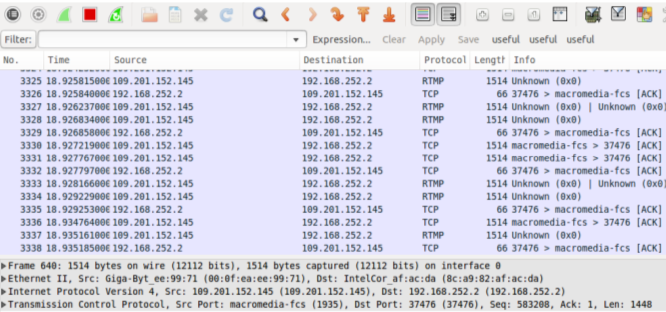
\includegraphics[scale=0.77]{wireshark.png}
	\caption{A sample Wireshark capture on our interface.
			 You can see a streaming TCP connection in the capture.}
\end{figure}
I would capture the destination interface for my packets.
This is very useful as I can see whether my rules accurately work in real time.
I can then replicate my test with a dumped pcap file that Wireshark generates.
The testing then also remains contained to a single machine.
This way, I will not have to deal much with external network rules. \par

However, after looking at the self-study slides and various Piazza posts,
I was able to set up the virtual network interface. This will be used to
debug the ARP handling module I will try and set up by tomorrow. I will also be
using Wireshark to physically check packets arriving and exiting these interfaces 
to make sure my code works and has easy debugging. \par

\section{Progress}

Currently I am behind the amount of work I had done for the progess report 
before Thanksgiving break. I am still working to get myself up to that stage
and get some working implementation of the Firewall ready. I anticipate I will
be unable to finish given that there will be less than 24 hours to do an entire
semester's worth of project. However, I plan to get as many modular elements of
the firewall working so that it is relatively simple to put together. \par
I have most of my file handling interfaces ready to use. I would like to get
the ARP resolution protocol complete, as it is orthogonal in its dependencies
to the rest of the firewall and can be show to work. \par
Given time, I would like to show multiple rules in work between two set
interfaces. That is what I am hoping for in the best case. 

\end{document}